\documentclass{beamer}

\usepackage{menukeys}

\usetheme{Boadilla}

% Title
\title{Vim Lab}
\author{Ethan Wong}
\date{October 13, 2023}
\institute{Linux Users Group @ UIC}

\begin{document}
\begin{frame}
	\titlepage
\end{frame}

\begin{frame}{Table of Contents}
	\tableofcontents[pausesections]
\end{frame}

\section{Why Vim?}
\begin{frame}{Why Vim?}
	\begin{itemize}
		\item Simple and ubiquitous text editor 
		\item Usable in a \textit{terminal}
		\item Keyboard-centric, meaning that a mouse is
			\underline{optional}
		\item Vim's version of modal input is popular and commonly emulated
		\item Part of the POSIX standard!
	\end{itemize}
\end{frame}

\section{History}
\begin{frame}{Table of Contents}
	\tableofcontents[currentsection]
\end{frame}

\begin{frame}{History}
	\begin{columns}
		\begin{column}{0.5\textwidth}
			\begin{itemize}
				\item Vi(no -m) was created by Bill Joy in \textbf{1976} for the
					Second BSD.\footnotemark
					\pause

				\item It is the visual mode for the \texttt{ex}
					command line text editor.
					\pause

				\item Vi was created for remote editing over a \textit{300} baud
					modem, which transmitted text slower than you can read!
					\pause
			\end{itemize}
		\end{column}
		\begin{column}{0.5\textwidth}
			\begin{figure}
				\centering
				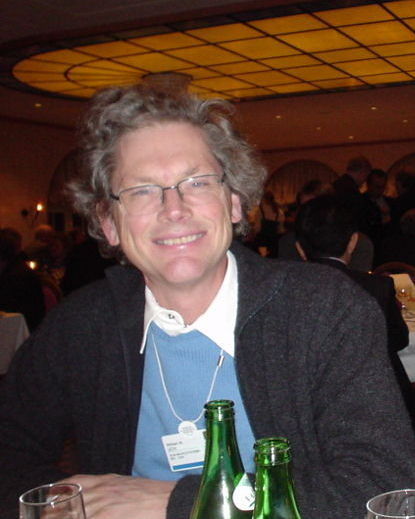
\includegraphics[width=0.5\textwidth]{bill_joy.jpg}
				\caption{Bill Joy, the creator of \texttt{vi}}
			\end{figure}
		\end{column}
	\end{columns}

	\footnotetext{\url{https://web.archive.org/web/20060701083055/http://web.cecs.pdx.edu/~kirkenda/joy84.html}}
\end{frame}

\begin{frame}{History}
	\begin{itemize}
		\item Vi iMproved (\texttt{vim}) was created by Bram Moolenaar
			in 1988 as a \textit{clone} of \texttt{vi}.
			\pause

		\item \texttt{vim} is a superset of \texttt{vi}, introducing new
			features such as syntax highlighting, undo/redo, screen
			splitting, and plugin support.
			\pause

		\item Like \texttt{vi}, \texttt{vim} has also been ported to a
			wide range of OS's.
			\pause

		\item Today, \texttt{vim} and its derivatives make up one of the
			most most popular text editor families.\footnotemark
	\end{itemize}

	\footnotetext{\url{https://survey.stackoverflow.co/2023/\#section-most-popular-technologies-integrated-development-environment}}
\end{frame}


\section{Basic Knowledge}
\begin{frame}{Table of Contents}
	\tableofcontents[currentsection]
\end{frame}

\subsection{Goals}
\begin{frame}{Goals}
	\begin{itemize}
		\item Learn how to switch between the different \textit{modes}
			of \texttt{vim}.
	\end{itemize}
\end{frame}

\subsection{Modes}
\begin{frame}{Modes}
	\texttt{vim} is known for a \textbf{modal} editing scheme.
	\pause

	What is modal editing?
	\pause

	In \texttt{vim}, various things that you typically do while editing text
	is split into different \textit{modes}.
	\pause

	\smallskip

	\begin{adjustbox}{max width=\textwidth}
		\begin{tabular}{ | l | l | l | }
			\hline
			\textbf{Mode} & \textbf{Purpose} & \textbf{How to Enter}\\
			\hline
			Normal & Move around and manipulate
			\textit{existing} text & Default, can return to
			by pressing \keys{\escwin} in other modes\\
			\hline
			Insert & Allows you to type text like in any standard
			editor & \keys{i}, \keys{a}, \keys{x}, \keys{c},
			\keys{o}, among others in Normal mode\\
			\hline
			Visual & Allows you to select regions of text as if you
			were using a mouse & \keys{v}, \keys{\shift + v},
			\keys{\ctrl + v} in Normal mode\\
			\hline
			Command & Allows you to execute commands like save and
			exit & \keys{:} in Normal mode\\
			\hline
		\end{tabular}
	\end{adjustbox}
	\smallskip
	\pause

	There are other additional modes that \texttt{vim} has out-of-the-box,
	but these are the basics.
	\pause

	Why should editing be split into modes?
\end{frame}

\subsection{Keybinds}
\begin{frame}{Keybinds}
	Modes allow for \texttt{vim} perform actions using simple and easy to
	remember keystroke sequences! \pause These are known as mmemonics!
	\pause

	\begin{exampleblock}{Example}
		Navigating can be done with \keys{h}, \keys{j}, \keys{k},
		\keys{l}. Which corrispond to \keys{\arrowkeyleft},
		\keys{\arrowkeydown}, \keys{\arrowkeyup}, \keys{\arrowkeyright}
		respectively.\footnote{People consider using the arrow keys in
		\texttt{vim} a cardinal sin.}
		\pause

		This allows you to keep your hands on the home-row of your
		keyboard (especially good if you are a touch-typist)!
	\end{exampleblock}
	\pause

	\begin{exampleblock}{Example 2}
		Additionally, 
	\end{exampleblock}
\end{frame}

\section{Crash Course}
\begin{frame}{Table of Contents}
	\tableofcontents[currentsection]
\end{frame}

\end{document}

% vim: set tw=80:
